\documentclass{article}

\usepackage{mathpartir}
\usepackage{amssymb}
\usepackage{graphicx}
\RequirePackage{algorithm}
\RequirePackage[noend]{algpseudocode}

\newcommand{\mod}{\mathrel{\mathrm{mod}}}
\newcommand{\imm}{\mathtt{imm}}
\newcommand{\mut}{\mathtt{mut}}
\newcommand{\funcall}[2]{{#1}\mathjs{(}{#2}\mathjs{)}}
\newcommand{\paren}[1]{\mathjs{(}{#1}\mathjs{)}}
\newcommand{\dom}{\mathit{dom}}
\newcommand{\funtype}{\mathit{fun}\mbox{-}\mathit{type}}
\newcommand{\vartype}{\mathit{var}\mbox{-}\mathit{type}}
\newcommand{\rettype}{\mathit{return}\mbox{-}\mathit{type}}
\newcommand{\imptype}{\mathit{import}\mbox{-}\mathit{type}}
\newcommand{\stdtype}{\mathit{std}\mbox{-}\mathit{type}}
\newcommand{\funty}[2]{({#1}) \rightarrow {#2}}
\newcommand{\seq}[1]{\overline{{#1}}}
\newcommand{\mathjs}[1]{\mbox{\texttt{{#1}}}}
\newcommand{\mathjssm}[1]{\mbox{\texttt{\scriptsize {#1}}}}
\newcommand{\return}[1]{\mathjs{return }{#1}\mathjs{;}}
\newcommand{\fun}[3]{\mathjs{function }{#1}\mathjs{(}{#2}\mathjs{) \char123{} }{#3}\mathjs{ \char125{}}}
\newcommand{\ternary}[3]{{#1}\,\mathjs{?}\,{#2}\,\mathjs{:}{#3}}
\newcommand{\afun}[2]{\mathjs{function}\mathjs{(}{#1}\mathjs{) \char123{} }{#2}\mathjs{ \char125{}}}
\newcommand{\var}[1]{\mathjs{var }{#1}\mathjs{;}}
\newcommand{\rel}[1]{\scriptsize [\textsc{#1}]}
\newcommand\defeq{\stackrel{\mbox{\tiny def}}{=}}
\newcommand{\while}[2]{\mathjs{while (}{#1}\mathjs{) }{#2}}
\newcommand{\dowhile}[2]{\mathjs{do }{#1}\mathjs{ while (}{#2}\mathjs{);}}
\newcommand{\for}[4]{\mathjs{for (}{#1}\mathjs{; }{#2}\mathjs{; }{#3}\mathjs{) }{#4}}
\newcommand{\switch}[2]{\mathjs{switch (}{#1}\mathjs{) \char123{} }{#2}\mathjs{ \char125{}}}
\newcommand{\switchdef}[3]{\mathjs{switch (}{#1}\mathjs{) \char123{} }{#2}\mathjs{ default:}\,{#3}\mathjs{ \char125{}}}
\newcommand{\brk}{\mathjs{break;}}
\newcommand{\brkl}[1]{\mathjs{break }{#1}\mathjs{;}}
\newcommand{\cont}{\mathjs{continue;}}
\newcommand{\contl}[1]{\mathjs{continue }{#1}\mathjs{;}}
\newcommand{\lab}[2]{{#1}\mathjs{:}\,{#2}}
\newcommand{\ifone}[2]{\mathjs{if (}{#1}\mathjs{) }{#2}}
\newcommand{\iftwo}[3]{\mathjs{if (}{#1}\mathjs{) }{#2}\mathjs{ else }{#3}}
\newcommand{\block}[1]{\mathjs{\char123{} }{#1}\mathjs{ \char125{}}}
\newcommand{\ok}{\mathrm{\mathbf{ok}}}
\newcommand{\rulebreak}{\vspace{.1in}\\}
\newcommand{\bit}{\mathtt{bit}}
\newcommand{\unsigned}{\mathtt{unsigned}}
\newcommand{\intsm}{\mathjssm{intish}}
\newcommand{\doublesm}{\mathjssm{doublish}}
\newcommand{\signed}{\mathtt{signed}}
\newcommand{\fixnum}{\mathtt{fixnum}}
\newcommand{\double}{\mathtt{double}}
\newcommand{\view}[2]{\mathtt{view}^{#1}_{#2}}
\newcommand{\extern}{\mathtt{extern}}
\newcommand{\unk}{\mathtt{unknown}}
\newcommand{\str}{\mathtt{string}}
\newcommand{\undef}{\mathtt{undefined}}
\newcommand{\void}{\mathtt{void}}
\newcommand{\nul}{\mathtt{null}}
\newcommand{\num}{\mathtt{number}}
\newcommand{\obj}{\mathtt{object}}
\newcommand{\mustret}{\mathsf{return}}
\newcommand{\seqcomp}{\mathrel{;}}
\newcommand{\getprop}[2]{{#1}\mathjs{[}{#2}\mathjs{]}}
\newcommand{\getpropsm}[2]{{#1}\mathjssm{[}{#2}\mathjssm{]}}
\newcommand{\longlong}[2]{\mathjs{[}{#1},{#2}\mathjs{]}}
\newcommand{\toint}[1]{\mathjs{\~{}\~{}}{#1}}
\newcommand{\todouble}[1]{\mathjs{+}{#1}}
\renewcommand{\int}{\mathtt{int}}
\newcommand{\dword}{\mathtt{bits64}}
\newcommand{\function}{\mathtt{function}}
\newcommand{\union}[2]{{#1}\mathrel{|}{#2}}
\newcommand{\boolish}{\mathtt{boolish}}
\newcommand{\floor}{\mathtt{floor}}
\newcommand{\imul}{\mathtt{imul}}
\newcommand{\intish}{\mathtt{intish}}
\newcommand{\doublish}{\mathtt{doublish}}
\newcommand{\Fun}{\mathtt{Function}}

\newcommand{\progjudge}[1]{\vdash {#1}\ \ok}
\newcommand{\impjudge}[5]{{#1};{#2};{#3};{#4} \vdash {#5}\ \ok}
\newcommand{\iejudge}[4]{{#1};{#2} \vdash {#3} : {#4}}
\newcommand{\fnjudge}[2]{{#1} \vdash {#2}\ \ok}
\newcommand{\expjudge}[2]{{#1} \vdash {#2}\ \ok}
\newcommand{\stmtjudge}[5]{{#1};{#2} \vdash {#3} : {#4} / {#5}}
\newcommand{\exprjudge}[4]{{#1};{#2} \vdash {#3} : {#4}}
\newcommand{\stmtretjudge}[2]{\vdash {#1} \hookrightarrow {#2}}
\newcommand{\sjudge}[4]{{#1};{#2};{#3} \vdash {#4}\ \ok}

\newcommand{\returns}{\mathit{returns}}
\newcommand{\breaks}{\mathit{breaks}}

\begin{document}

\title{\texttt{asm.js}: a High-Performance Subset of JavaScript}
\author{Dave Herman, Luke Wagner, and Alon Zakai}
\maketitle

\section{Introduction}

This document describes a formal definition of a subset of the
JavaScript programming language that can be used as a high-performance
compiler target language. This sublanguage or dialect, which we call
$\mathjs{asm.js}$, effectively describes a safe virtual machine for
memory-unsafe languages such as C and C++.

Because $\mathjs{asm.js}$ is a proper subset of JavaScript, both
syntactically and semantically, the language is fully defined by a
static {\it validation} judgment, which yields a predicate that
determines whether a given JavaScript program is or is not in the
subset. No specification of a dynamic semantics is needed, since the
behavior of an $\mathjs{asm.js}$ program is simply defined by its
behavior as a JavaScript program.

\subsection{Overview}

The unit of compilation/validation of $\mathjs{asm.js}$ is the
$\mathjs{asm.js}$ {\it module}, which takes the form of a closed
JavaScript function beginning with the {\it prologue
directive}~\cite{es5}:
\[
\mathjs{"use asm";}
\]
The presence of this directive serves two purposes. First, it allows
JavaScript engines that wish to provide specialized optimizations for
$\mathjs{asm.js}$ to efficiently recognize that the module should be
validated as an $\mathjs{asm.js}$, without the need for complex,
heuristic or concurrent recognition logic. (Since validation requires
a non-trivial traversal of the body of the module, it is likely too
expensive to speculatively validate {\it all} JavaScript code during
JIT compilation.) Second, by requiring the programmer or code
generator to state the intention explicitly that the code should be
recognized as $\mathjs{asm.js}$, it allows user agents to report
validation errors or performance faults to developer consoles.

An $\mathjs{asm.js}$ module takes three optional parameters: a global
object, containing standard ECMAScript libraries, an {\it FFI object},
containing custom imported functions and constants from external
JavaScript, and a JavaScript $\mathjs{ArrayBuffer}$ representing a
virtualized memory. The module can provide different views of the
buffer by using typed array wrappers imported from the environment:
\begin{verbatim}
function mod(global, foreign, buffer) {
    "use asm";

    var HEAP_I32 = new global.Int32Array(buffer);
    var HEAP_F64 = new global.Float64Array(buffer);
    // ...
}
\end{verbatim}

The body of an $\mathjs{asm.js}$ module consists of any number of
function definitions, followed by an {\it export clause}:
\[
\return{\mathjs{\char123{} foo:\,f, bar:\,g \char125{}}}
\]
If a module only exports a single function, it can do so directly,
without the object literal:
\[
\return{\mathjs{foo}}
\]

\subsection{Types}

The $\mathjs{asm.js}$ language is statically typed: every function,
variable, and expression has a statically predictable type, according
to a type hierarchy covering a subset of JavaScript values (see
Section~\ref{sec:types}). Variables, parameters, and functions are
provided with an explicit type bound through a stylized use of
JavaScript coercions. This technique was pioneered by the Emscripten
compiler~\cite{emscripten}, and is now used by a number of compilers
that target JavaScript~\cite{mandreel,lljs}.

For example, the following is a simple function from integers to
integers:
\begin{verbatim}
function id(x) {
    x = x|0;
    return x|0;
}
\end{verbatim}
Even though JavaScript provides only double-precision floating-point
numbers (doubles) in its data model, the $\mathjs{asm.js}$ type system
enforces that 32-bit integer values---a strict subset of
doubles---never overflow to larger doubles. This allows optimizing
compilers to represent these values as unboxed integers in 32-bit
registers or memory.

Again following the practice established by Emscripten, it is possible
to do integer operations such as arithmetic and conditionals by means
of coercions:
\begin{verbatim}
function add1(x) {
    x = x|0;
    return ((x|0)+1)|0;
}
\end{verbatim}
While the JavaScript semantics dictates that the addition may overflow
to a larger number than a 32-bit integer, the outer coercion ensures
that the entire expression results in a 32-bit integer---the same
integer that would be produced by a signed, 32-bit addition in a
typical assembly language. The $\mathjs{asm.js}$ type system thus
ensures that integer operations can be efficiently compiled by
optimizing JavaScript engines to predictable machine instructions.

\subsection{Validation, linking, and execution}

The $\mathjs{asm.js}$ validator is defined as a static type system,
which can be performed by an optimizing JavaScript engine at the time
the module is parsed by the JavaScript engine. (If compilation time is
a concern, it can be delayed to runtime by hiding the source code in a
string and passed to $\mathjs{eval}$ or the $\mathjs{Function}$
constructor.) During this phase, any static validation errors can be
reported to a developer console.

After a $\mathjs{asm.js}$ module is compiled, its evaluation produces
a closure with an empty lexical environment. The module can be {\it
linked} by calling the function with an object representing the
imported environment and an optional buffer:
\begin{verbatim}
function mod(global, foreign, buffer) {
    "use asm";
    // ...
    return { f: foo, g: bar };
}

var foreign = {
    consoleDotLog: console.log,
    // ...
};

var buffer = new ArrayBuffer(0x100000);

// link the module
var m = mod(window, foreign, buffer);
\end{verbatim}

This linking phase may need to perform additional, dynamic
validation. In particular, dynamic validation can fail if, for
example, the $\mathjs{Int32Array}$ function passed in through the
environment does not turn out to construct a proper typed array
(thereby defeating typed array-based optimizations).

The resulting module object provides access to the exported
$\mathjs{asm.js}$ functions, which have been fully validated (both
statically and dynamically) and optimized.

\subsection{Notation conventions}

The following notation conventions are used in this document. Optional
items in a grammar are presented in $[\mbox{square
brackets}]$. Sequences are presented with a $\seq{\mbox{horizontal
overbar}}$. The empty sequence is denoted by $\epsilon$. Integers and
integer literals are ranged over by the metavariables $i, j$;
these may also serve as sequence indices, in which case they are
natural numbers. Natural numbers are otherwise ranged over by the
metavariables $m, n$. Floating-point literals are ranged over by the
metavariable $r$.

\subsection{Document outline}

The remainder of this document proceeds as follows.
%% FIXME: outline

\section{Abstract syntax}

This section specifies the abstract syntax of $\mathjs{asm.js}$. The
grammar is presented with concrete syntax for conciseness and
readability, but should be read as describing the subset of abstract
syntax trees produced by a standard JavaScript parser.

We make the following assumptions about canonicalization of
$\mathjs{asm.js}$ abstract syntax trees:
\begin{enumerate}
\item Parentheses are ignored in the AST. This allows parentheses to
  be left out of any of the formal definitions of this spec.

\item Empty statements ($\mathjs{;}$) are ignored in the AST. This
  allows empty statements to be left out of any of the formal
  definitions of this spec.

\item The identifiers $\mathjs{arguments}$ and $\mathjs{eval}$ do not
  appear in $\mathjs{asm.js}$ programs. If either of these identifiers
  appears anywhere, static validation must fail.
\end{enumerate}

In various places in this document, the meta-variables $f$, $g$, $x$,
$y$, and $z$ are used to range over JavaScript identifiers.

We syntactically distinguish integer literals $i, j$ from
floating-point literals $r$. A floating-point literal is a JavaScript
number literal that contains a $\mathjs{.}$ character.

\subsection{Modules}

An $\mathjs{asm.js}$ module has the following syntax:
\[
\begin{array}{rcl}
\mathit{mod} & ::= & \mathjs{function }[f]\mathjs{(}[\mathit{global}[, \mathit{foreign}[, \mathit{buffer}]]]\mathjs{) \char123{}} \\
             &     & \qquad\mathjs{"use asm";} \\
             &     & \qquad\seq{\var{\seq{x \mathjs{ = } \mathit{imp}}}} \\
             &     & \qquad\seq{\mathit{fn}_g} \\
             &     & \qquad\seq{\var{\seq{y \mathjs{ = } v}}} \\
             &     & \qquad\mathit{exp} \\
             &     & \mathjs{\char125{}} \\
%%                     \fun{[m]}{[g[, e[, b]]]}{\mathjs{"use asm"; } \seq{\mathit{imp}_x}\ \seq{\mathit{fn}_f}\ \seq{\var{\seq{y \mathjs{ = } v}}}\ \mathit{exp}}
\end{array}
\]
The syntax consists of:
\begin{enumerate}
\item an optional module name;
\item up to three optional parameters;
\item a $\mathjs{"use asm";}$ prologue directive;
\item a sequence of import statements;
\item a sequence of function declarations;
\item a sequence of global variable declarations; and
\item a single export statement.
\end{enumerate}

An import expression is either an FFI function binding, a
type-annotated (coerced) FFI value, or a heap view:
\[
\begin{array}{rcl}
\mathit{imp}  & ::= & \mathit{global}\mathjs{.}x \\
              &  |  & \mathit{global}\mathjs{.Math.}x \\
              &  |  & \mathjs{new }\funcall{\mathit{global}\mathjs{.}x}{\mathit{buffer}} \\
              &  |  & \mathit{foreign}\mathjs{.}x\mathjs{|0} \\
              &  |  & \mathjs{+}\mathit{foreign}\mathjs{.}x \\
              &  |  & \mathit{foreign}\mathjs{.}x \\
\end{array}
\]
(We assume that the metavariables $\mathit{global}$,
$\mathit{foreign}$, and $\mathit{buffer}$ stand for fixed variables
names used consistently throughout the imports.)

A function declaration has the following syntax:
\[
\mathit{fn}_f ::= \fun{f}{\seq{x}}{\seq{x\mathjs{ = }\mathit{ann}_x\mathjs{;}}\ \seq{\var{\seq{y\mathjs{ = }v}}}\ \mathit{ss}}
\]
The syntax consists of type annotations for the parameters, a sequence
of local variable declarations, and a sequence of statements.

Type annotations are either $\int$ or $\double$ coercions:
\[
\mathit{ann}_x ::= x\mathjs{|0} ~|~ \todouble{x}
\]

An export statement returns either a single function or an object
literal containing multiple functions:
\[
\begin{array}{rcl}
\mathit{exp}    & ::= & \return{f} \\
                &  |  & \return{\mathjs{\char123{} } \seq{x \mathjs{:} f} \mathjs{ \char125{}}} \\
\end{array}
\]

\subsection{Statements}

The set of legal statements in $\mathjs{asm.js}$ includes blocks,
expression statements, conditionals, returns, loops, $\mathjs{switch}$
blocks, $\mathjs{break}$ and $\mathjs{continue}$, and labeled
statements:
\[
\begin{array}{rcl}
s & ::= & \block{\mathit{ss}} \\
  &  |  & e\mathjs{;} \\
  &  |  & \ifone{e}{s} \\
  &  |  & \iftwo{e}{s}{s} \\
  &  |  & \return{[\mathit{re}]} \\
  &  |  & \while{e}{s} \\
  &  |  & \dowhile{s}{e} \\
  &  |  & \for{[e]}{[e]}{[e]}{s} \\
  &  |  & \switch{e}{\seq{c}\ [d]} \\
  &  |  & \brkl{[\mathit{lab}]} \\
  &  |  & \contl{[\mathit{lab}]} \\
  &  |  & \lab{\mathit{lab}}{s} \\
\\
\mathit{ss} & ::= & \seq{s} \\
\end{array}
\]

Return arguments always have their type explicitly manifest: either a
$\signed$ or $\double$ coercion or a literal:
\[
\mathit{re} ::= e\mathjs{|0} ~|~ \todouble{e} ~|~ v
\]

The contents of $\mathjs{switch}$ blocks are restricted: in addition
to requiring the (optional) $\mathjs{default}$ clause to be the last
clause, each $\mathjs{case}$ clause is syntactically restricted to
contain only literal values:
\[
\begin{array}{rcl}
c & ::= & \mathjs{case }v\mathjs{:}\,\mathit{ss} \\
d & ::= & \mathjs{default:}\,\mathit{ss} \\
\mathit{cd} & ::= & c ~|~ d \\
\end{array}
\]

\subsection{Expressions}

Expressions include literals, lvalues, assignments, function calls,
unary expressions, binary expressions, and sequence expressions:
\[
\begin{array}{rcl}
e & ::= & v \\
  &  |  & \mathit{lval} \\
  &  |  & \mathit{lval}\mathjs{ = }e \\
  &  |  & \funcall{f}{\seq{e}} \\
  &  |  & \mathit{unop}\ e \\
  &  |  & e\ \mathit{binop}\ e \\
  &  |  & \ternary{e}{e}{e} \\
  &  |  & \paren{\seq{e}} \\
\\
\mathit{unop} & ::= & \mathjs{+} ~|~ \mathjs{\~{}} ~|~ \mathjs{!} \\
\\
\mathit{binop} & ::= & \mathjs{+} ~|~ \mathjs{-} ~|~ \mathjs{*} ~|~ \mathjs{/} ~|~ \mathjs{\%} \\
               &  |  & \mathjs{|} ~|~ \mathjs{\&} ~|~ \mathjs{\^{}} ~|~ \mathjs{<<} ~|~ \mathjs{>>} ~|~ \mathjs{>>>} \\
               &  |  & \mathjs{<} ~|~ \mathjs{<=} ~|~ \mathjs{>} ~|~ \mathjs{>=} ~|~ \mathjs{!=} ~|~ \mathjs{==} \\
\end{array}
\]

Literals are either doubles or integers:
\[
v ::= r ~|~ i
\]

Lvalues are either variables or typed array dereference
expressions. The latter requires a mask to force the byte offset into
a valid range and a shift to convert the offset into a proper index
for the size of the typed array.
\[
\mathit{lval} ::= x ~|~ \getprop{x}{i} ~|~ \getprop{x}{e\mathjs{ \& }\mathit{mask}} ~|~ \getprop{x}{\paren{e\mathjs{ \& }\mathit{mask}}\mathjs{ >> }i}
\]
The $\mathit{mask}$ is a non-negative integer $2^k - 1$ where $k \in
[3, 31]$.  The same $\mathit{mask}$ must be used consistently
throughout the program.

\section{Types}
\label{sec:types}

The $\mathjs{asm.js}$ validator relies on a static type system that
classifies and constraints the syntax beyond the grammar.

\subsection{Expression types}

The set of {\it expression types} classifies the results of expression
evaluation and constrains the allowable values of variables.
\[
\begin{array}{rcl}
\sigma, \tau & ::= & \fixnum ~|~ \signed ~|~ \unsigned ~|~ \int ~|~ \intish \\
             &  |  & \double ~|~ \doublish ~|~ \extern ~|~ \unk ~|~ \void \\
%% \sigma, \tau & ::= & \double ~|~ \signed ~|~ \unsigned ~|~ \fixnum ~|~ \extern \\
%%              &  |  & \bit ~|~ \int ~|~ \boolish ~|~ \intish ~|~ \void ~|~ \unk \\
\end{array}
\]

These types are arranged in a subtyping hierarchy, defined by:
\[
\begin{array}{rcl}
\fixnum            & <: & \signed, \unsigned \\
\signed, \unsigned & <: & \int, \extern \\
\double            & <: & \extern, \doublish \\
\unk               & <: & \intish, \doublish \\
\int               & <: & \intish \\
\end{array}
\]

Figure~\ref{fig:subtypes} depicts this subtyping hierarchy
visually. Note that some types are presented in white boxes and others
in gray boxes. The white boxes represent types that may escape into
external JavaScript; the gray types are internal to the
$\mathjs{asm.js}$ module and cannot escape. This allows an optimizing
implementation to use unboxed representations that would otherwise be
illegal. What follows is an explanation of each type.

\begin{figure}[tb]
\centering
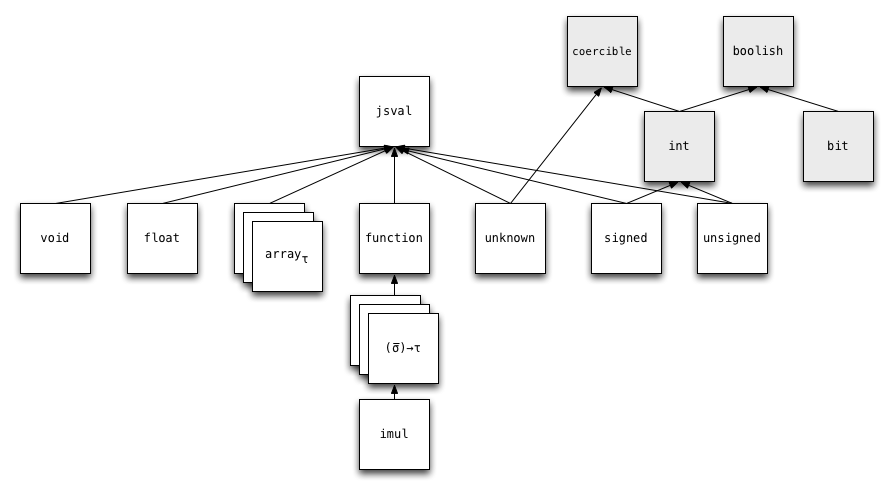
\includegraphics[scale=0.5]{subtypes}
\caption{The hierarchy of expression types.}
\label{fig:subtypes}
\end{figure}

\subsubsection*{The $\extern$ type}

This abstract type represents the root of all types that can escape
back into ordinary JavaScript. Any type that is a subtype of $\extern$
must carry enough information in its internal representation in an
optimizing virtual machine to faithfully convert back into a dynamic
JavaScript value.

\subsubsection*{The $\double$ type}

This is the type of double-precision floating-point values. An
optimizing engine can represent these as unboxed 64-bit floats. If
they escape into external JavaScript they must of course be wrapped
back up as JavaScript values according to the JavaScript engine's
value representation.

\subsubsection*{The $\signed$ and $\unsigned$ types}

These are the types of signed and unsigned 32-bit integers,
respectively. For an optimizing engine, their representation can be
the same: an unboxed 32-bit integer. If a value escapes into external
JavaScript, the sign is used to determine which JavaScript value it
represents. For example, the bit pattern $\mathjs{0xffffffff}$
represents either the JavaScript value $\mathjs{-1}$ or
$\mathjs{4294967295}$, depending on the signedness of the type.

\subsubsection*{The $\fixnum$ type}

This type represents integers in the range $[0, 2^{31})$, which are
both valid signed and unsigned integers. Literals in this range are
given the type $\fixnum$ rather than $\signed$ or $\unsigned$, since
either way they have the same representation as an unboxed 32-bit
integer.

\subsubsection*{The $\int$ type}

This is the type of 32-bit integers whose sign is not known. Again,
optimizing engines can represent them as unboxed 32-bit integers. But
because the sign is not known, they cannot be allowed to escape to
external JavaScript, as it is impossible to determine exactly which
JavaScript value they represent. While this might not seem like a very
useful type, the JavaScript bitwise coercions can be used to force an
$\int$ value back to $\signed$ or $\unsigned$ without any loss of
data.

The conditional operators also produce the $\int$ type, even though,
according to the JavaScript semantics, they produce boolean
values. Since boolean values convert to the integer values
$\mathjs{0}$ and $\mathjs{1}$, it is sound to represent the boolean
values in an optimizing engine as integers, even while allowing them
to be stored in integer values and passed to integer
arithmetic. Similarly, integer values can be treated as ``boolish'' in
JavaScript when used in conditional contexts, so it is safe to store
boolean values as unboxed integers even when being used in the test
expression of an $\mathjs{if}$ statement and the like.

\subsubsection*{The $\intish$ type}

The JavaScript arithmetic operations can be performed on 32-bit
integer values, but their results may produce non-integer values. For
example, addition and subtraction can overflow to large numbers that
exceed the 32-bit integer range, and integer division can produce a
non-integer value. However, if the result is coerced back to an
integer, the resulting arithmetic operation behaves identically to the
typical corresponding machine operation (i.e., integer addition,
subtraction, or division). The $\intish$ type represents the result of
a JavaScript integer artihmetic operation that must be coerced back to
integer with an explicit coercion. Because this type can only be used
as an argument to a coercion (or silently ignored in an expression
statement), $\mathjs{asm.js}$ integer arithmetic can always be
implemented in an optimizing engine by the machine integer artithmetic
operations.

The one arithmetic operation that does not quite fit into this story
is multiplication. Multiplying two large integers can results in a
large enough double that some lower bits of precision are lost, so
that coercing the result back to integer does {\it not} behave
identically to the machine operation. The use of the proposed ES6
$\mathjs{Math.imul}$ function~\cite{imul} as an FFI function is
recommended as the proper means of implementing integer
multiplication.

In short:

\begin{quote}
The $\intish$ type represents the result of integer operations that
must be dropped or immediately coerced via $\mathit{ToInt32}$ or
$\mathit{ToUint32}$.
\end{quote}

\subsubsection*{The $\doublish$ type}

Similarly, the $\doublish$ type represents operations that are
expected to produce a $\double$ but may produce additional junk that
must be coerced back to a number via $\mathit{ToNumber}$. In
particular, reading from the typed array may produce
$\mathjs{undefined}$, and calling FFI functions may produce an
arbitrary JavaScript value. Thus:

\begin{quote}
The $\doublish$ type represents the result of numeric operations that
must be dropped or immediately coerced via $\mathit{ToNumber}$.
\end{quote}

\subsubsection*{The $\unk$ type}

Calling an external JavaScript function through the FFI results in an
arbitrary JavaScript value. Because $\mathjs{asm.js}$ is designed to
avoid dealing with general values, the result must be coerced to one
of the other types before it can be used. The $\unk$ type represents
one of these result values before being coerced to an integer or
double.

\subsubsection*{The $\void$ type}

A function that returns $\mathjs{undefined}$ is considered to have the
$\void$ result type. The $\mathjs{undefined}$ value is not actually a
first-class value in $\mathjs{asm.js}$. It can only be ignored via an
expression statement. This avoids having to represent it at all as
data.

\subsection{Global types}

Validation tracks the types not only of expressions and local
variables but also global variables, FFI imports, and functions. In
addition to variables of expression type, globals may also be typed
array views on the module's buffer, imported FFI constants and
functions, and functions defined in the $\mathjs{asm.js}$ module.
\[
\gamma ::= \tau ~|~ \view{n}{\tau} ~|~ (\funty{\seq{\sigma}}{\tau}) \land \cdots \land (\funty{\seq{\sigma'}}{\tau'}) ~|~ \Fun
\]

The type of a typed array tracks the number of bytes per element and
the elements' value type ($\intish$ or $\doublish$). A function type
may be overloaded to allow different parameter types, potentially
providing different result types for each overloading.

\subsection{Operator types}

Every operator, unary or binary, has an overloaded function type.
This overloading corresponds to the different machine operations used
in an optimizing engine to implement the various cases. Whereas
JavaScript generally needs to choose the behavior of operators
dynamically, $\mathjs{asm.js}$ makes it possible to resolve the
overloaded operators statically based on the types of the operands.

The types of the arithmetic operators are as follows:
\[
\begin{array}{rcc@{\ }l}
\mathjs{+}       & : &       & \funty{\double, \double}{\double} \\
%                 &   & \land & \funty{\int, \int}{\intish} \\
\mathjs{-}       & : &       & \funty{\doublish, \doublish}{\double} \\
%                 &   & \land & \funty{\int, \int}{\intish} \\
\mathjs{*}       & : &       & \funty{\doublish, \doublish}{\double} \\
\mathjs{/}       & : &       & \funty{\doublish, \doublish}{\double} \\
                 &   & \land & \funty{\signed, \signed}{\intish}  \\
                 &   & \land & \funty{\unsigned, \unsigned}{\intish} \\
\mathjs{\%}      & : &       & \funty{\doublish, \doublish}{\double} \\
                 &   & \land & \funty{\signed, \signed}{\int}  \\
                 &   & \land & \funty{\unsigned, \unsigned}{\int} \\
\end{array}
\]
%% Note that some operations produce the type $\intish$, indicating that
%% their result must be immediately coerced back to an integer. Note also
%% that some operations accept $\doublish$ arguments, because they coerce
%% them immediately with $\mathit{ToNumber}$. (This is not the case for
%% the binary $\mathjs{+}$ operator, which therefore requires its
%% argument to be a true $\double$.)
The type of addition and subtraction only deals with floating-point
arithmetic; for integer addition and subtraction see
Section~\ref{sec:exprjudge}. Similarly, the $\mathjs{*}$ operator
provides only floating-point multiplication; integer multiplication
can be implemented via the $\imul$ function. The $\mathjs{/}$ operator
does provide both floating-point and integer division; for the latter
it produces the type $\intish$, which requires a coercion via the
bitwise operators to produce the proper integer result. The
$\mathjs{\%}$ operator works as either a floating-point or integer
operator and produces the correct result without any need for a
coercion.

The bitwise operators are one of only two places in the language that
can consume an $\intish$ expression. Every one of these operators can
be composed with the arithmetic operators to produce the correct
behavior of integer arithmetic.
\[
\begin{array}{rcc@{\ }l}
\mathjs{|}, \mathjs{\&}, \mathjs{\^{}}, \mathjs{<<}, \mathjs{>>}
                 & : &       & \funty{\intish, \intish}{\signed} \\
\mathjs{>>>}     & : &       & \funty{\intish, \intish}{\unsigned} \\
\end{array}
\]

The conditional operators rely on the sign of their input and produce
a boolean result:
\[
\begin{array}{rcc@{\ }l}
\mathjs{<}, \mathjs{<=}, \mathjs{>}, \mathjs{>=}, \mathjs{==}, \mathjs{!=}
                 & : &       & \funty{\signed, \signed}{\int} \\
                 &   & \land & \funty{\unsigned, \unsigned}{\int} \\
                 &   & \land & \funty{\double, \double}{\int} \\
\end{array}
\]

Finally, the unary operators have function types as well; unary
operations can also serve as coercions: the $\mathjs{+}$ operator
converts integers and the results of typed array reads and FFI calls
to $\double$, and the $\mathjs{\~{}}$ operator can be used to coerce
$\intish$ expressions, similar to the two-argument bitwise operators.
\[
\begin{array}{rcc@{\ }l}
\mathjs{+}       & : &       & \funty{\signed}{\double} \\
                 &   & \land & \funty{\unsigned}{\double} \\
                 &   & \land & \funty{\doublish}{\double} \\
\mathjs{-}       & : &       & \funty{\int}{\intish} \\
                 &   & \land & \funty{\doublish}{\double} \\
\mathjs{\~{}}    & : &       & \funty{\intish}{\signed} \\
\end{array}
\]

\section{Validation}

This section describes the $\mathjs{asm.js}$ validation process, which
is essentially a static type system.

\subsection{Standard libraries}

The JavaScript $\mathjs{Math}$ API is recognized as a typed standard
library; most of its functions are allowed as imports with the same
name and are given appropriate function types. These functions must be
passed into the import environment under their respective names (e.g.,
$\mathjs{Math.sin}$ under the name $g\mathjs{.Math.sin}$). Building in
support for these standard functions allows optimizing engines to
build special support for them---particularly the $\imul$ operation,
which can be implemented with hardware multiplication instructions.
\[
\begin{array}{rcl}
M(\mathtt{acos}), M(\mathtt{asin}), M(\mathtt{atan}) & = & \funty{\doublish}{\double} \\
M(\mathtt{cos}), M(\mathtt{sin}), M(\mathtt{tan})    & = & \funty{\doublish}{\double} \\
M(\mathtt{ceil}), M(\mathtt{floor})                  & = & \funty{\doublish}{\double} \\
M(\mathtt{exp}), M(\mathtt{log}), M(\mathtt{sqrt})   & = & \funty{\doublish}{\double} \\
M(\mathtt{abs}) & =     & \funty{\signed}{\unsigned} \\
                & \land & \funty{\doublish}{\double} \\
M(\mathtt{atan2}), M(\mathtt{pow}) & = & \funty{\doublish, \doublish}{\double} \\
M(\imul) & = & \funty{\int, \int}{\signed} \\
M(\mathtt{random}) & = & \funty{}{\double} \\
M(\mathtt{E}) & = & \double \\
M(\mathtt{LN10}), M(\mathtt{LN2}), M(\mathtt{LOG2E}), M(\mathtt{LOG10E}) & = & \double \\
M(\mathtt{PI}) & = & \double \\
M(\mathtt{SQRT1\_2}), M(\mathtt{SQRT2}) & = & \double \\
\end{array}
\]

\subsection{View types}

The typed array constructors are also recognized as imports in the
import environment, each under its standard name. Calling the various
typed arrays constructors on the buffer produces typed array views of
various types.
\[
\begin{array}{rcl}
V(\mathtt{Uint8Array}), V(\mathtt{Int8Array})   & = & \view{1}{\intsm} \\
V(\mathtt{Uint16Array}), V(\mathtt{Int16Array}) & = & \view{2}{\intsm} \\
V(\mathtt{Uint32Array}), V(\mathtt{Int32Array}) & = & \view{4}{\intsm} \\
V(\mathtt{Float32Array})                        & = & \view{4}{\doublesm} \\
V(\mathtt{Float64Array})                        & = & \view{8}{\doublesm} \\
\end{array}
\]

\subsection{Global constants}

\[
\begin{array}{rcl}
G(\mathtt{Infinity}), G(\mathtt{NaN}) & = & \double \\
\end{array}
\]

\subsection{Annotations}

Type annotations are provided in the form of explicit
coercions. Variables in $\mathjs{asm.js}$ are always taken to have the
type $\double$ or $\int$, never $\signed$ or $\unsigned$. This is
because they are intended to be representable as unboxed 32-bit words
in memory or registers, which are agnostic about what sign to
interpret the bits with.

\[
\begin{array}{rcl}
\vartype(\todouble{x}), \vartype(r) & = & \double \\
\vartype(x\mathjs{|0}), \vartype(i) & = & \int \mbox{ $(-2^{31} \leq i < 2^{32})$}
\end{array}
\]

Function return types are determined by explicit coercions in their
return statements. Function return types are always explicit about
their sign so that they can be exported to external JavaScript.

\[
\begin{array}{rcl}
\rettype(\todouble{e}), \rettype(r) & = & \double \\
\rettype(e\mathjs{|0}), \rettype(i) & = & \signed \mbox{ $(-2^{31} \leq i < 2^{31})$} \\
\rettype(\epsilon)                  & = & \void \\
\end{array}
\]

The type of a function can be extracted by looking at its parameter
annotations and return statements.

\[
\begin{array}{l}
\funtype(\fun{f}{\seq{x}}{\seq{x\mathjs{ = }\mathit{ann}_x\mathjs{;}}\ \seq{\var{\seq{y\mathjs{ = }v}}}\ \mathit{ss}\ \return{[\mathit{re}]}}) = \funty{\seq{\sigma}}{\tau} \\
\qquad \mbox{where } \forall i . \vartype(\mathit{ann}_{x_i}) = \sigma_i \\
\qquad \mbox{and } \rettype([\mathit{re}]) = \tau \\
\funtype(\fun{f}{\seq{x}}{\seq{x\mathjs{ = }\mathit{ann}_x\mathjs{;}}\ \seq{\var{\seq{y\mathjs{ = }v}}}\ \mathit{ss}\ s}) = \funty{\seq{\sigma}}{\void} \\
\qquad \mbox{where } \forall i . \vartype(\mathit{ann}_{x_i}) = \sigma_i \\
\qquad \mbox{and } s \not= \return{[\mathit{re}]} \\
\funtype(\fun{f}{\seq{x}}{\seq{x\mathjs{ = }\mathit{ann}_x\mathjs{;}}\ \seq{\var{\seq{y\mathjs{ = }v}}}\ \epsilon}) = \funty{\seq{\sigma}}{\void} \\
\qquad \mbox{where } \forall i . \vartype(\mathit{ann}_{x_i}) = \sigma_i \\
\end{array}
\]

The types of import expressions are determined by the standard library
metafunctions $G$, $M$, and $V$ or by their coercion. A foreign import
with no coercion is assumed to be a function.

\[
\begin{array}{l}
\imptype(\mathit{global}\mathjs{.}x) = G(x) \\
\imptype(\mathit{global}\mathjs{.Math.}x) = M(x) \\
\imptype(\mathjs{new }\funcall{\mathit{global}\mathjs{.}x}{\mathit{buffer}}) = V(y) \\
\imptype(\mathit{foreign}\mathjs{.}x\mathjs{|0}) = \signed \\
\imptype(\mathjs{+}\mathit{foreign}\mathjs{.}x) = \double \\
\imptype(\mathit{foreign}\mathjs{.}x) = \Fun \\
\end{array}
\]

\subsection{Module validation}

Module validation takes an $\mathjs{asm.js}$ module and constructs a
{\it global environment} $\Delta$, which is used to track the types of
all globals: imports, buffer views, global variables, and functions.
\[
\begin{array}{rcl}
\mu    & ::= & \mut ~|~ \imm \\
\Delta & ::= & \{ \seq{x : \mu\,\gamma} \} \\
\end{array}
\]
Validation then uses this environment to check the imports, exports,
and function definitions.

\newsavebox{\modjudge}
\begin{lrbox}{\modjudge}
\begin{minipage}[t]{3in}
\vspace{-.25in}
\[
\begin{array}{rll}
       & \mathjs{function }[f]\mathjs{(}[\mathit{global}[, \mathit{foreign}[, \mathit{buffer}]]]\mathjs{) \char123{}} \\
       & \qquad\mathjs{"use asm";} \\
       & \qquad\seq{\var{\seq{x \mathjs{ = } \mathit{imp}}}} \\
\vdash & \qquad\seq{\mathit{fn}_g} & \ok \\
       & \qquad\seq{\var{\seq{y \mathjs{ = } v}}} \\
       & \qquad\mathit{exp} \\
       & \mathjs{\char125{}} \\
\end{array}
\]
\end{minipage}
\end{lrbox}

\[
\begin{array}{c}
\multicolumn{1}{r}{\fbox{$\progjudge{\mathit{mod}}$}}
\rulebreak
\inferrule* [lab=\rel{T-Module}]
  {\Delta = \{ \seq{x : \imm\,\imptype(\mathit{imp})}, \seq{g : \imm\,\funtype(\mathit{fn}_g)}, \seq{y : \mut\,\vartype(v)} \} \\\\
   %%\forall i . \impjudge{[g]}{[e]}{[b]}{\Delta}{\mathit{imp}_x} \\
   \seq{x}, \seq{y}, \seq{g}, [f], [\mathit{global}], [\mathit{foreign}], [\mathit{buffer}]\ \mbox{distinct} \\
   \forall i . \fnjudge{\Delta}{\mathit{fn}_f} \\
   \forall i . \expjudge{\Delta}{\mathit{exp}}}
  {\usebox{\modjudge}}
%  {\progjudge{\fun{[m]}{[g[, e[, b]]}{\mathjs{"use asm";}\ \seq{\mathit{imp}_x}\ \seq{\mathit{fn}_f}\ \seq{\var{\seq{y \mathjs{ = } v}}}\ \mathit{exp}}}}
\end{array}
\]

For simplicity of the specification, we leave as an assumption that
the same $\mathit{global}$, $\mathit{foreign}$, and $\mathit{buffer}$
variables are used consistently throughout the module. An actual
validator must check this assumption. Similarly, we assume the
existence of a single $\mathit{mask}$ constant used throughout the
module, which a real validator would have to check.

%% \subsection{Import validation}

%% Declarations in the import section of an $\mathjs{asm.js}$ module can
%% be known library functions, unknown FFI functions, typed array views,
%% or imported constants.

%% \[
%% \begin{array}{c}
%% \multicolumn{1}{r}{\fbox{$\impjudge{[g]}{[e]}{[b]}{\Delta}{\mathit{imp}}$}}
%% \rulebreak
%% \inferrule* [lab=\rel{T-ImportStd}]
%%   {\iejudge{[g]}{[e]}{\mathit{ie}}{\Delta(x)}}
%%   {\impjudge{[g]}{[e]}{[b]}{\Delta}{\var{x \mathjs{ = } \mathit{ie}}}}
%% \qquad
%% \inferrule* [lab=\rel{T-ImportFFI}]
%%   {\iejudge{[g]}{[e]}{\mathit{ie}}{\epsilon} \\\\
%%    \Delta(x) = \Fun}
%%   {\impjudge{[g]}{[e]}{[b]}{\Delta}{\var{x \mathjs{ = } \mathit{ie}}}}
%% \\ \\
%% \inferrule* [lab=\rel{T-ImportInt}]
%%   {\iejudge{[g]}{[e]}{\mathit{ie}}{\tau} \\\\
%%    \tau <: \intish \\
%%    \Delta(x) = \signed}
%%   {\impjudge{[g]}{[e]}{[b]}{\Delta}{\var{x \mathjs{ = } \mathit{ie}\mathjs{|0}}}}
%% \qquad
%% \inferrule* [lab=\rel{T-ImportDouble}]
%%   {\iejudge{[g]}{[e]}{\mathit{ie}}{\tau} \\\\
%%    \tau <: \doublish \\
%%    \Delta(x) = \double}
%%   {\impjudge{[g]}{[e]}{[b]}{\Delta}{\var{x \mathjs{ = +}\mathit{ie}}}}
%% \\ \\
%% \inferrule* [lab=\rel{T-ImportView}]
%%   {\Delta(x) = V(y)}
%%   {\impjudge{g}{[e]}{b}{\Delta}{\var{x \mathjs{ = new } g\mathjs{.}y(b)}}}
%% %% \\ \\
%% %% \inferrule* [lab=\rel{T-ImportStd}]
%% %%   {\Delta(x) = M(y)}
%% %%   {\impjudge{[g]}{[e]}{[b]}{\Delta}{\var{x \mathjs{ = } e\mathjs{.}y}}}
%% %% \qquad
%% %% \inferrule* [lab=\rel{T-ImportFFI}]
%% %%   {y \not\in\dom(M), \dom(A) \\\\
%% %%    \Delta(x) = \Fun}
%% %%   {\impjudge{[g]}{e}{[b]}{\Delta}{\var{x \mathjs{ = } c\mathjs{.}y}}}
%% %% \\ \\
%% %% \inferrule* [lab=\rel{T-View}]
%% %%   {\Delta(x) = \view{n}{A(y)}}
%% %%   {\impjudge{[g]}{e}{b}{\Delta}{\var{x \mathjs{ = new } c\mathjs{.}y(b)}}}
%% %% \\ \\
%% %% \inferrule* [lab=\rel{T-ImportInt}]
%% %%   {\Delta(x) = \int}
%% %%   {\impjudge{[g]}{e}{[b]}{\Delta}{\var{x \mathjs{ = }c\mathjs{.}y\mathjs{|0}}}}
%% %% \qquad
%% %% \inferrule* [lab=\rel{T-ImportDouble}]
%% %%   {\Delta(x) = \double}
%% %%   {\impjudge{[g]}{e}{[b]}{\Delta}{\var{x \mathjs{ = +}c\mathjs{.}y}}}
%% \end{array}
%% \]

%% \[
%% \begin{array}{c}
%% \multicolumn{1}{r}{\fbox{$\iejudge{[g]}{[e]}{\mathit{ie}}{[\gamma]}$}}
%% \rulebreak
%% \inferrule* [lab=\rel{T-Global}]
%%   {y \in \dom(G)}
%%   {\iejudge{g}{[e]}{g\mathjs{.}y}{G(y)}}
%% \qquad
%% \inferrule* [lab=\rel{T-Math}]
%%   {y \in \dom(M)}
%%   {\iejudge{g}{[e]}{g\mathjs{.Math.}y}{M(y)}}
%% \qquad
%% \inferrule* [lab=\rel{T-FFI}]
%%   { }
%%   {\iejudge{[g]}{e}{e\mathjs{.}y}{\epsilon}}
%% \end{array}
%% \]

\subsection{Function validation}

Function validation proceeds in several steps. First, a local
environment is constructed with bindings for the parameters and local
variables, based on their annotations and initializers,
respectively. Next, the body of the function is checked in this
environment. Finally, if the function has a non-$\void$ return type,
the body is checked to ensure that all control flow paths definitely
return a value (see Section~\ref{sec:cfa}).

\[
\begin{array}{c}
\multicolumn{1}{r}{\fbox{$\fnjudge{\Delta}{\mathit{fn}}$}}
\rulebreak
\inferrule* [lab=\rel{T-Function}]
  {\seq{x}, \seq{y}\ \mbox{distinct} \\
   \Delta(f) = \imm\,\funty{\seq{\sigma}}{\tau} \\
   \seq{\sigma} = \seq{\vartype(\mathit{ann}_x)} \\\\
   \sjudge{\Delta}{\{ \seq{x : \sigma}, \seq{y : \vartype(v)} \}}{\tau}{\mathit{ss}}}
  {\fnjudge{\Delta}{\fun{f}{\seq{x}}{\seq{x\mathjs{ = }\mathit{ann}_x\mathjs{;}}\ \seq{\var{\seq{y\mathjs{ = }v}}}\ \mathit{ss}}}}
\end{array}
\]

\subsection{Export validation}

Export validation ensures that all exports are functions.

\[
\begin{array}{c}
\multicolumn{1}{r}{\fbox{$\expjudge{\Delta}{\mathit{exp}}$}}
\rulebreak
\inferrule* [lab=\rel{T-Singleton}]
  {\Delta(f) = \imm\,\funty{\seq{\sigma}}{\tau}}
  {\expjudge{\Delta}{\return{f}}}
\qquad
\inferrule* [lab=\rel{T-Module}]
  {\forall f . \Delta(f) = \imm\,\funty{\seq{\sigma}}{\tau}}
  {\expjudge{\Delta}{\return{\mathjs{\char123{} } \seq{x \mathjs{:} f} \mathjs{ \char125{}}}}}
\end{array}
\]

\subsection{Statement list validation}

\[
\begin{array}{c}
\multicolumn{1}{r}{\fbox{$\sjudge{\Delta}{\Gamma}{\tau}{\mathit{ss}}$}}
\rulebreak
\inferrule* [lab=\rel{T-Statements}]
  {\forall i . \sjudge{\Delta}{\Gamma}{\tau}{s_i}}
  {\sjudge{\Delta}{\Gamma}{\tau}{\seq{s}}}
\end{array}
\]


\subsection{Statement validation}

\newsavebox{\switchcontrol}
\begin{lrbox}{\switchcontrol}
\begin{minipage}[t]{2.87in}
\vspace{-.25in}
\[
\varepsilon = \left\{ \begin{array}{ll}
                      \mustret & \mbox{if}\ \varepsilon_n = \mustret \land \forall i . \varepsilon_i \cup \emptyset = \emptyset \\
                      \bigcup \varepsilon_i - \{ \epsilon \} & \mbox{otherwise}
                      \end{array} \right.
\]
\end{minipage}
\end{lrbox}

\[
\begin{array}{c}
\multicolumn{1}{r}{\fbox{$\sjudge{\Delta}{\Gamma}{\tau}{s}$}}
\rulebreak
\inferrule* [lab=\rel{T-Block}]
  {\sjudge{\Delta}{\Gamma}{\tau}{\mathit{ss}}}
  {\sjudge{\Delta}{\Gamma}{\tau}{\block{\mathit{ss}}}}
\qquad
\inferrule* [lab=\rel{T-ExprStmt}]
  {\exprjudge{\Delta}{\Gamma}{e}{\sigma}}
  {\sjudge{\Delta}{\Gamma}{\tau}{e\mathjs{;}}}
\qquad
\inferrule* [lab=\rel{T-EmptyStatement}]
  { }
  {\sjudge{\Delta}{\Gamma}{\tau}{\mathjs{;}}}
\\ \\
\inferrule* [lab=\rel{T-If}]
  {\exprjudge{\Delta}{\Gamma}{e}{\boolish} \\\\
   \sjudge{\Delta}{\Gamma}{\tau}{s}}
  {\sjudge{\Delta}{\Gamma}{\tau}{\ifone{e}{s}}}
\qquad
\inferrule* [lab=\rel{T-IfElse}]
  {\exprjudge{\Delta}{\Gamma}{e}{\boolish} \\\\
   \sjudge{\Delta}{\Gamma}{\tau}{s_1} \\
   \sjudge{\Delta}{\Gamma}{\tau}{s_2}}
  {\sjudge{\Delta}{\Gamma}{\tau}{\iftwo{e}{s_1}{s_2}}}
\\ \\
\inferrule* [lab=\rel{T-ReturnExpr}]
  {\exprjudge{\Delta}{\Gamma}{\mathit{re}}{\tau} \\\\
   \rettype(\mathit{re}) = \tau}
  {\sjudge{\Delta}{\Gamma}{\tau}{\return{\mathit{re}}}}
%% \qquad
%% \inferrule* [lab=\rel{T-ReturnDouble}]
%%   {\exprjudge{\Delta}{\Gamma}{e}{\double}}
%%   {\sjudge{\Delta}{\Gamma}{\double}{\return{\mathjs{+}e}}}
\qquad
\inferrule* [lab=\rel{T-ReturnVoid}]
  { }
  {\sjudge{\Delta}{\Gamma}{\void}{\mathtt{return;}}}
\\ \\
\inferrule* [lab=\rel{T-While}]
  {\exprjudge{\Delta}{\Gamma}{e}{\int} \\\\
   \sjudge{\Delta}{\Gamma}{\tau}{s}}
  {\sjudge{\Delta}{\Gamma}{\tau}{\while{e}{s}}}
\qquad
\inferrule* [lab=\rel{T-DoWhile}]
  {\sjudge{\Delta}{\Gamma}{\tau}{s} \\\\
   \exprjudge{\Delta}{\Gamma}{e}{\int}}
  {\sjudge{\Delta}{\Gamma}{\tau}{\dowhile{s}{e}}}
\\ \\
\inferrule* [lab=\rel{T-For}]
  {[\exprjudge{\Delta}{\Gamma}{e_1}{\sigma_1}] \\
   [\exprjudge{\Delta}{\Gamma}{e_2}{\int}] \\
   [\exprjudge{\Delta}{\Gamma}{e_3}{\sigma_3}] \\\\
   \sjudge{\Delta}{\Gamma}{\tau}{s}}
  {\sjudge{\Delta}{\Gamma}{\tau}{\for{[e_1]}{[e_2]}{[e_3]}{s}}}
\\ \\
\inferrule* [lab=\rel{T-Break}]
  { }
  {\sjudge{\Delta}{\Gamma}{\tau}{\brkl{[\mathit{lab}]}}}
\qquad
\inferrule* [lab=\rel{T-Continue}]
  { }
  {\sjudge{\Delta}{\Gamma}{\tau}{\contl{[\mathit{lab}]}}}
\qquad
\inferrule* [lab=\rel{T-Label}]
  {\sjudge{\Delta}{\Gamma}{\tau}{s}}
  {\sjudge{\Delta}{\Gamma}{\tau}{\lab{\mathit{lab}}{s}}}
\\ \\
\inferrule* [lab=\rel{T-Switch}]
  {\exprjudge{\Delta}{\Gamma}{e}{\sigma} \\
   \sigma \in \{ \signed, \unsigned \} \\
   \forall i . \exprjudge{\Delta}{\Gamma}{v_i}{\sigma} \\\\
   \forall i . \sjudge{\Delta}{\Gamma}{\tau}{\mathit{ss}_i} \\
   [\sjudge{\Delta}{\Gamma}{\tau}{\mathit{ss}}]}
  {\sjudge{\Delta}{\Gamma}{\tau}{\switch{e}{\seq{\mathjs{case }v_i\mathjs{:}\,\mathit{ss}_i}\ [\mathjs{default:}\,\mathit{ss}]}}}
\end{array}
\]

\subsection{Case validation}

\[
\begin{array}{c}
\multicolumn{1}{r}{\fbox{$\sjudge{\Delta}{\Gamma}{\tau}{\mathit{cd}}$}}
\rulebreak
\inferrule* [lab=\rel{T-Case}]
  {\sjudge{\Delta}{\Gamma}{\tau}{\mathit{ss}}}
  {\sjudge{\Delta}{\Gamma}{\tau}{\mathjs{case }v\mathjs{:}\,\mathit{ss}}}
\qquad
\inferrule* [lab=\rel{T-Default}]
  {\sjudge{\Delta}{\Gamma}{\tau}{\mathit{ss}}}
  {\sjudge{\Delta}{\Gamma}{\tau}{\mathjs{default:}\,\mathit{ss}}}
\end{array}
\]

%% \subsection{Must-return analysis}
%% \label{sec:cfa}

%% \[
%% \begin{array}{rcl}
%% \breaks(\seq{s}) & = & \bigcup_i \breaks(s_i) \\
%% \breaks(\block{\mathit{ss}}) & = & \breaks(\mathit{ss}) \\
%% \breaks(\ifone{e}{s}) & = & \breaks(s) \\
%% \breaks(\iftwo{e}{s_1}{s_2}) & = & \breaks(s_1) \cup \breaks(s_2) \\
%% \breaks(\while{e}{s}) & = & \breaks(s) - \{ \epsilon \} \\
%% \breaks(\dowhile{s}{e}) & = & \breaks(s) - \{ \epsilon \} \\
%% \breaks(\for{[e_1]}{[e_2]}{[e_3]}{s}) & = & \breaks(s) - \{ \epsilon \} \\
%% \breaks(\brk) & = & \{ \epsilon \} \\
%% \breaks(\brkl{\mathit{lab}}) & = & \{ \mathit{lab} \} \\
%% \breaks(\lab{\mathit{lab}}{s}) & = & \breaks(s) - \{ \mathit{lab} \} \\
%% \breaks(\switch{e}{\seq{\mathit{cd}}}) & = & \bigcup_i \breaks(\mathit{cd}_i) - \{ \epsilon \} \\
%% \breaks(s) \mbox{ (otherwise)} & = & \emptyset \\
%% \breaks(\mathjs{case }v\mathjs{:}\,\mathit{ss}) & = & \breaks(\mathit{ss}) \\
%% \breaks(\mathjs{default:}\,\mathit{ss}) & = & \breaks(\mathit{ss}) \\
%% \end{array}
%% \]

%% \[
%% \begin{array}{l}
%% \returns(\seq{s}) \\
%% \qquad \mbox{if } \returns(s_m) \land \forall i < m . \breaks(s_m) = \emptyset \mbox{ for some } m \\
%% \returns(\block{\mathit{ss}}) \\
%% \qquad \mbox{if } \returns(ss) \\
%% \returns(\iftwo{e}{s_1}{s_2}) \\
%% \qquad \mbox{if } \returns(s_1) \land \returns(s_2) \\
%% \returns(\dowhile{s}{e}) \\
%% \qquad \mbox{if } \returns(s) \\
%% \returns(\switch{e}{\seq{\mathit{cd}}}) \\
%% \qquad \mbox{if } \returns(cd_n) \land \forall i . \breaks(cd_i) = \emptyset \\
%% \returns(\mathjs{case }v\mathjs{:}\,\mathit{ss}) \\
%% \qquad \mbox{if } \returns(\mathit{ss}) \\
%% \returns(\mathjs{default:}\,\mathit{ss}) \\
%% \qquad \mbox{if } \returns(\mathit{ss})
%% \end{array}
%% \]

\subsection{Expression validation}
\label{sec:exprjudge}

\[
(\Delta\cdot\Gamma)(x) = \left\{\begin{array}{ll}
                                \Gamma(x) & \mbox{if}\ x \in\dom(\Gamma) \\
                                \gamma & \mbox{if}\ \Delta(x) = \mu\,\gamma \\
                                \end{array} \right.
\]

\[
\begin{array}{lr}
\mbox{Expression validation} & \hfil \fbox{$\exprjudge{\Delta}{\Gamma}{e}{\tau}$}
\rulebreak
\multicolumn{2}{c}{
\begin{array}{c}
\inferrule* [lab=\rel{T-Signed}]
  {-2^{31} \leq i < 0}
  {\exprjudge{\Delta}{\Gamma}{i}{\signed}}
\qquad
\inferrule* [lab=\rel{T-Fixnum}]
  {0 \leq i < 2^{31}}
  {\exprjudge{\Delta}{\Gamma}{i}{\fixnum}}
\qquad
\inferrule* [lab=\rel{T-Unsigned}]
  {2^{31} \leq i < 2^{32}}
  {\exprjudge{\Delta}{\Gamma}{i}{\unsigned}}
\\ \\
\inferrule* [lab=\rel{T-Double}]
  { }
  {\exprjudge{\Delta}{\Gamma}{r}{\double}}
\qquad
\inferrule* [lab=\rel{T-VarRef}]
  {(\Delta\cdot\Gamma)(x) = \tau}
  {\exprjudge{\Delta}{\Gamma}{x}{\tau}}
\\ \\
\inferrule* [lab=\rel{T-SetLocal}]
  {\exprjudge{\Delta}{\Gamma}{e}{\tau} \\
   \tau <: \Gamma(x)}
  {\exprjudge{\Delta}{\Gamma}{x\mathjs{ = }e}{\tau}}
\qquad
\inferrule* [lab=\rel{T-SetGlobal}]
  {x \not\in\dom(\Gamma) \\
   \Delta(x) = \mut\,\sigma \\\\
   \exprjudge{\Delta}{\Gamma}{e}{\tau} \\
   \tau <: \sigma}
  {\exprjudge{\Delta}{\Gamma}{x\mathjs{ = }e}{\tau}}
\\ \\
\inferrule* [lab=\rel{T-LoadImm}]
  {(\Delta\cdot\Gamma)(x) = \view{n}{\tau} \\\\
   i \equiv 0 \mod n \\
   0 \leq i \leq \mathit{mask} \\\\
   \exprjudge{\Delta}{\Gamma}{e}{\intish}}
  {\exprjudge{\Delta}{\Gamma}{\getprop{x}{i}}{\tau}}
\qquad
\inferrule* [lab=\rel{T-StoreImm}]
  {(\Delta\cdot\Gamma)(x) = \view{n}{\tau} \\\\
   i \equiv 0 \mod n \\
   0 \leq i \leq \mathit{mask} \\\\
   \exprjudge{\Delta}{\Gamma}{e_1}{\intish} \\
   \exprjudge{\Delta}{\Gamma}{e_2}{\tau}}
  {\exprjudge{\Delta}{\Gamma}{\getprop{x}{i}\mathjs{ = }e_2}{\tau}}
\\ \\
\inferrule* [lab=\rel{T-LoadByte}]
  {(\Delta\cdot\Gamma)(x) = \view{1}{\intsm} \\\\
   \exprjudge{\Delta}{\Gamma}{e}{\intish}}
  {\exprjudge{\Delta}{\Gamma}{\getprop{x}{e\mathjs{ \& } \mathit{mask}}}{\tau}}
\qquad
\inferrule* [lab=\rel{T-StoreByte}]
  {(\Delta\cdot\Gamma)(x) = \view{1}{\intsm} \\\\
   \exprjudge{\Delta}{\Gamma}{e_1}{\intish} \\
   \exprjudge{\Delta}{\Gamma}{e_2}{\tau}}
  {\exprjudge{\Delta}{\Gamma}{\getprop{x}{e_1\mathjs{ \& } \mathit{mask}}\mathjs{ = }e_2}{\tau}}
\\ \\
\inferrule* [lab=\rel{T-Load}]
  {(\Delta\cdot\Gamma)(x) = \view{n}{\tau} \\\\
   \mathit{shift} = \log_2(n) \\
   n > 1 \\\\
   \exprjudge{\Delta}{\Gamma}{e}{\intish}}
  {\exprjudge{\Delta}{\Gamma}{\getprop{x}{\paren{e\mathjs{ \& } \mathit{mask}}\mathjs{ >> } \mathit{shift}}}{\tau}}
\qquad
\inferrule* [lab=\rel{T-Store}]
  {(\Delta\cdot\Gamma)(x) = \view{n}{\tau} \\\\
   \mathit{shift} = \log_2(n) \\
   n > 1 \\\\
   \exprjudge{\Delta}{\Gamma}{e_1}{\intish} \\
   \exprjudge{\Delta}{\Gamma}{e_2}{\tau}}
  {\exprjudge{\Delta}{\Gamma}{\getprop{x}{\paren{e_1\mathjs{ \& } \mathit{mask}}\mathjs{ >> } \mathit{shift}}\mathjs{ = }e_2}{\tau}}
\end{array}
}
\end{array}
\]

\[
\begin{array}{lr}
\mbox{Expression validation (cont'd)} & \hfil \fbox{$\exprjudge{\Delta}{\Gamma}{e}{\tau}$}
\rulebreak
\multicolumn{2}{c}{
\begin{array}{c}
\inferrule* [lab=\rel{T-FunCall}]
  {(\Delta\cdot\Gamma)(f) = \_ \land \funty{\seq{\sigma}}{\tau} \land \_ \\\\
   \forall i . \exprjudge{\Delta}{\Gamma}{e_i}{\sigma_i}}
  {\exprjudge{\Delta}{\Gamma}{\funcall{f}{\seq{e}}}{\tau}}
\qquad
\inferrule* [lab=\rel{T-FFICall}]
  {(\Delta\cdot\Gamma)(f) = \Fun \\\\
   %(\Delta\cdot\Gamma)(f) = \_ \land \funty{\ldots\sigma}{\tau} \land \_ \\\\
   \forall i . \exprjudge{\Delta}{\Gamma}{e_i}{\extern}}
  {\exprjudge{\Delta}{\Gamma}{\funcall{f}{\seq{e}}}{\unk}}
\\ \\
\inferrule* [lab=\rel{T-Unop}]
  {\mathit{unop} : \_ \land \funty{\sigma}{\tau} \land \_ \\\\
   \exprjudge{\Delta}{\Gamma}{e}{\sigma}}
  {\exprjudge{\Delta}{\Gamma}{\mathit{unop}\ e}{\tau}}
\qquad
\inferrule* [lab=\rel{T-Binop}]
  {\mathit{binop} : \_ \land \funty{\sigma_1, \sigma_2}{\tau} \land \_ \\\\
   \exprjudge{\Delta}{\Gamma}{e_1}{\sigma_1} \\
   \exprjudge{\Delta}{\Gamma}{e_2}{\sigma_2}}
  {\exprjudge{\Delta}{\Gamma}{e_1\ \mathit{binop}\ e_2}{\tau}}
\\ \\
\inferrule* [lab=\rel{T-Multiary}]
  {\forall i < n . \oplus_i \in \{ +, - \} \\
   n \leq 2^{20} \\\\
   \forall i \leq n . \exprjudge{\Delta}{\Gamma}{e_i}{\int}}
  {\exprjudge{\Delta}{\Gamma}{e_1 \oplus_1 \ldots \oplus_{n-1} e_n}{\intish}}
\qquad
\inferrule* [lab=\rel{T-Cond}]
  {\tau \in \{ \int, \double \} \\\\
   \exprjudge{\Delta}{\Gamma}{e_1}{\int} \\\\
   \exprjudge{\Delta}{\Gamma}{e_2}{\tau} \\
   \exprjudge{\Delta}{\Gamma}{e_3}{\tau}}
  {\exprjudge{\Delta}{\Gamma}{\ternary{e_1}{e_2}{e_3}}{\tau}}
\\ \\
\inferrule* [lab=\rel{T-Paren}]
  {\forall i \leq n . \exprjudge{\Delta}{\Gamma}{e_i}{\tau_i}}
  {\exprjudge{\Delta}{\Gamma}{\paren{\seq{e}}}{\tau_n}}
\qquad
\inferrule* [lab=\rel{T-Sub}]
  {\exprjudge{\Delta}{\Gamma}{e}{\sigma} \\
   \sigma <: \tau}
  {\exprjudge{\Delta}{\Gamma}{e}{\tau}}
\qquad
\inferrule* [lab=\rel{T-Cast}]
  {\exprjudge{\Delta}{\Gamma}{e}{\double}}
  {\exprjudge{\Delta}{\Gamma}{\mathjs{\~{}\~{}}e}{\signed}}
\end{array}
}
\end{array}
\]

\end{document}
